\chapter{METODOLOGIA}\label{chap:metodologia}

Este trabalho possui pesquisa aplicada. Para atingir nossos objetivos precisamos construir um sistema capaz de estimar a atitude e a posição de um corpo a partir de dados obtidos de um modelo específico de sensor inercial. Nesse desiderato planejamos estabelecer o sistema mais simples possível mas que seja flexível o bastante para avaliar os resultados ao final.

Para atender ao tema proposto, dividimos o trabalho em etapas:
\begin{itemize}
    \item Seleção de literatura com abordagens viáveis.
    \item Estudo dos manuais do produto, prototipagem e testes preliminares.
    \item Desenvolvimento de software.
    \item Testes de bancada para coleta de dados.
    \item Análise dos dados.
\end{itemize}

\section{Revisão de Literatura}

Após revisão abrangente, nos deparamos com métodos e abordagens bastante diversos para descrever a orientação de objetos e seus movimentos. Selecionamos as abordagens mais intuitivas e simples, que atendem ao objetivo de testar a viabilidade da aplicação desejada para os sensores. 

\section{Estudo do sensor, prototipagem, testes preliminares}

Utilizamos, inicialmente, um sensor inercial modelo MPU-6050 (Figura~\ref{fig:mpu6050-sensor-top}) anexado a uma Raspberry Pi 3B (Figuras~\ref{fig:mpu6050-board-top}~e~\ref{fig:mpu6050-proto-top}):
\begin{figure}[H]
    \centering
    \caption{Sensor MPU-6050 encapsulado}\label{fig:mpu6050-sensor-top}
    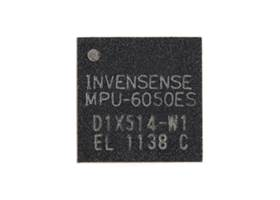
\includegraphics[width=0.5\textwidth]{figuras/mpu6050-sensor-top-straight.jpg}
    \fonte{o autor}
\end{figure}
A orientação dos sensores em relação ao encapsulamento obedece a regra da mão direita, conforme descrito na Figura~\ref{fig:mpu6050-diagram-axis}:
\begin{figure}[H]
    \centering
    \caption{Sensor MPU-6050 eixos em relação ao encapsulamento}\label{fig:mpu6050-diagram-axis}
    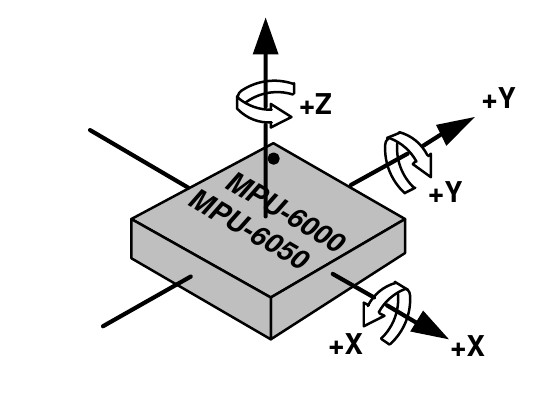
\includegraphics[width=0.5\textwidth]{figuras/mpu6050-diagram-axis.jpg}
    \fonte{\citeonline{mpu6050ps}}
\end{figure}
\begin{figure}[H]
    \centering
    \caption{Sensor MPU-6050 montado em placa módulo}\label{fig:mpu6050-board-top}
    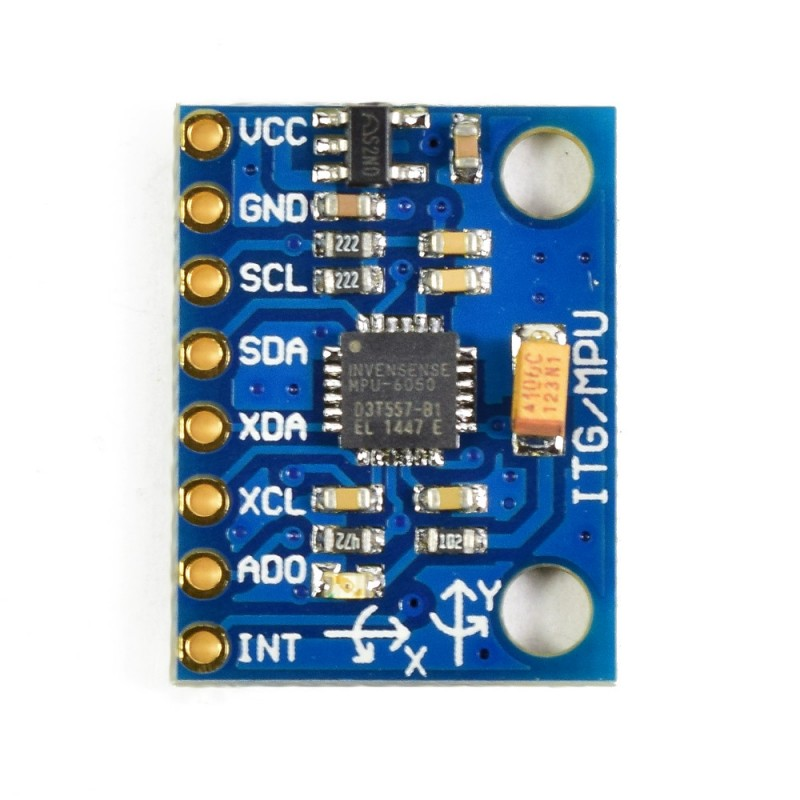
\includegraphics[width=0.5\textwidth]{figuras/mpu6050-board-top.jpg}
    \fonte{o autor}
\end{figure}
\begin{figure}[H]
    \centering
    \caption{Sensor MPU-6050 anexado à Raspberry Pi}\label{fig:mpu6050-proto-top}
    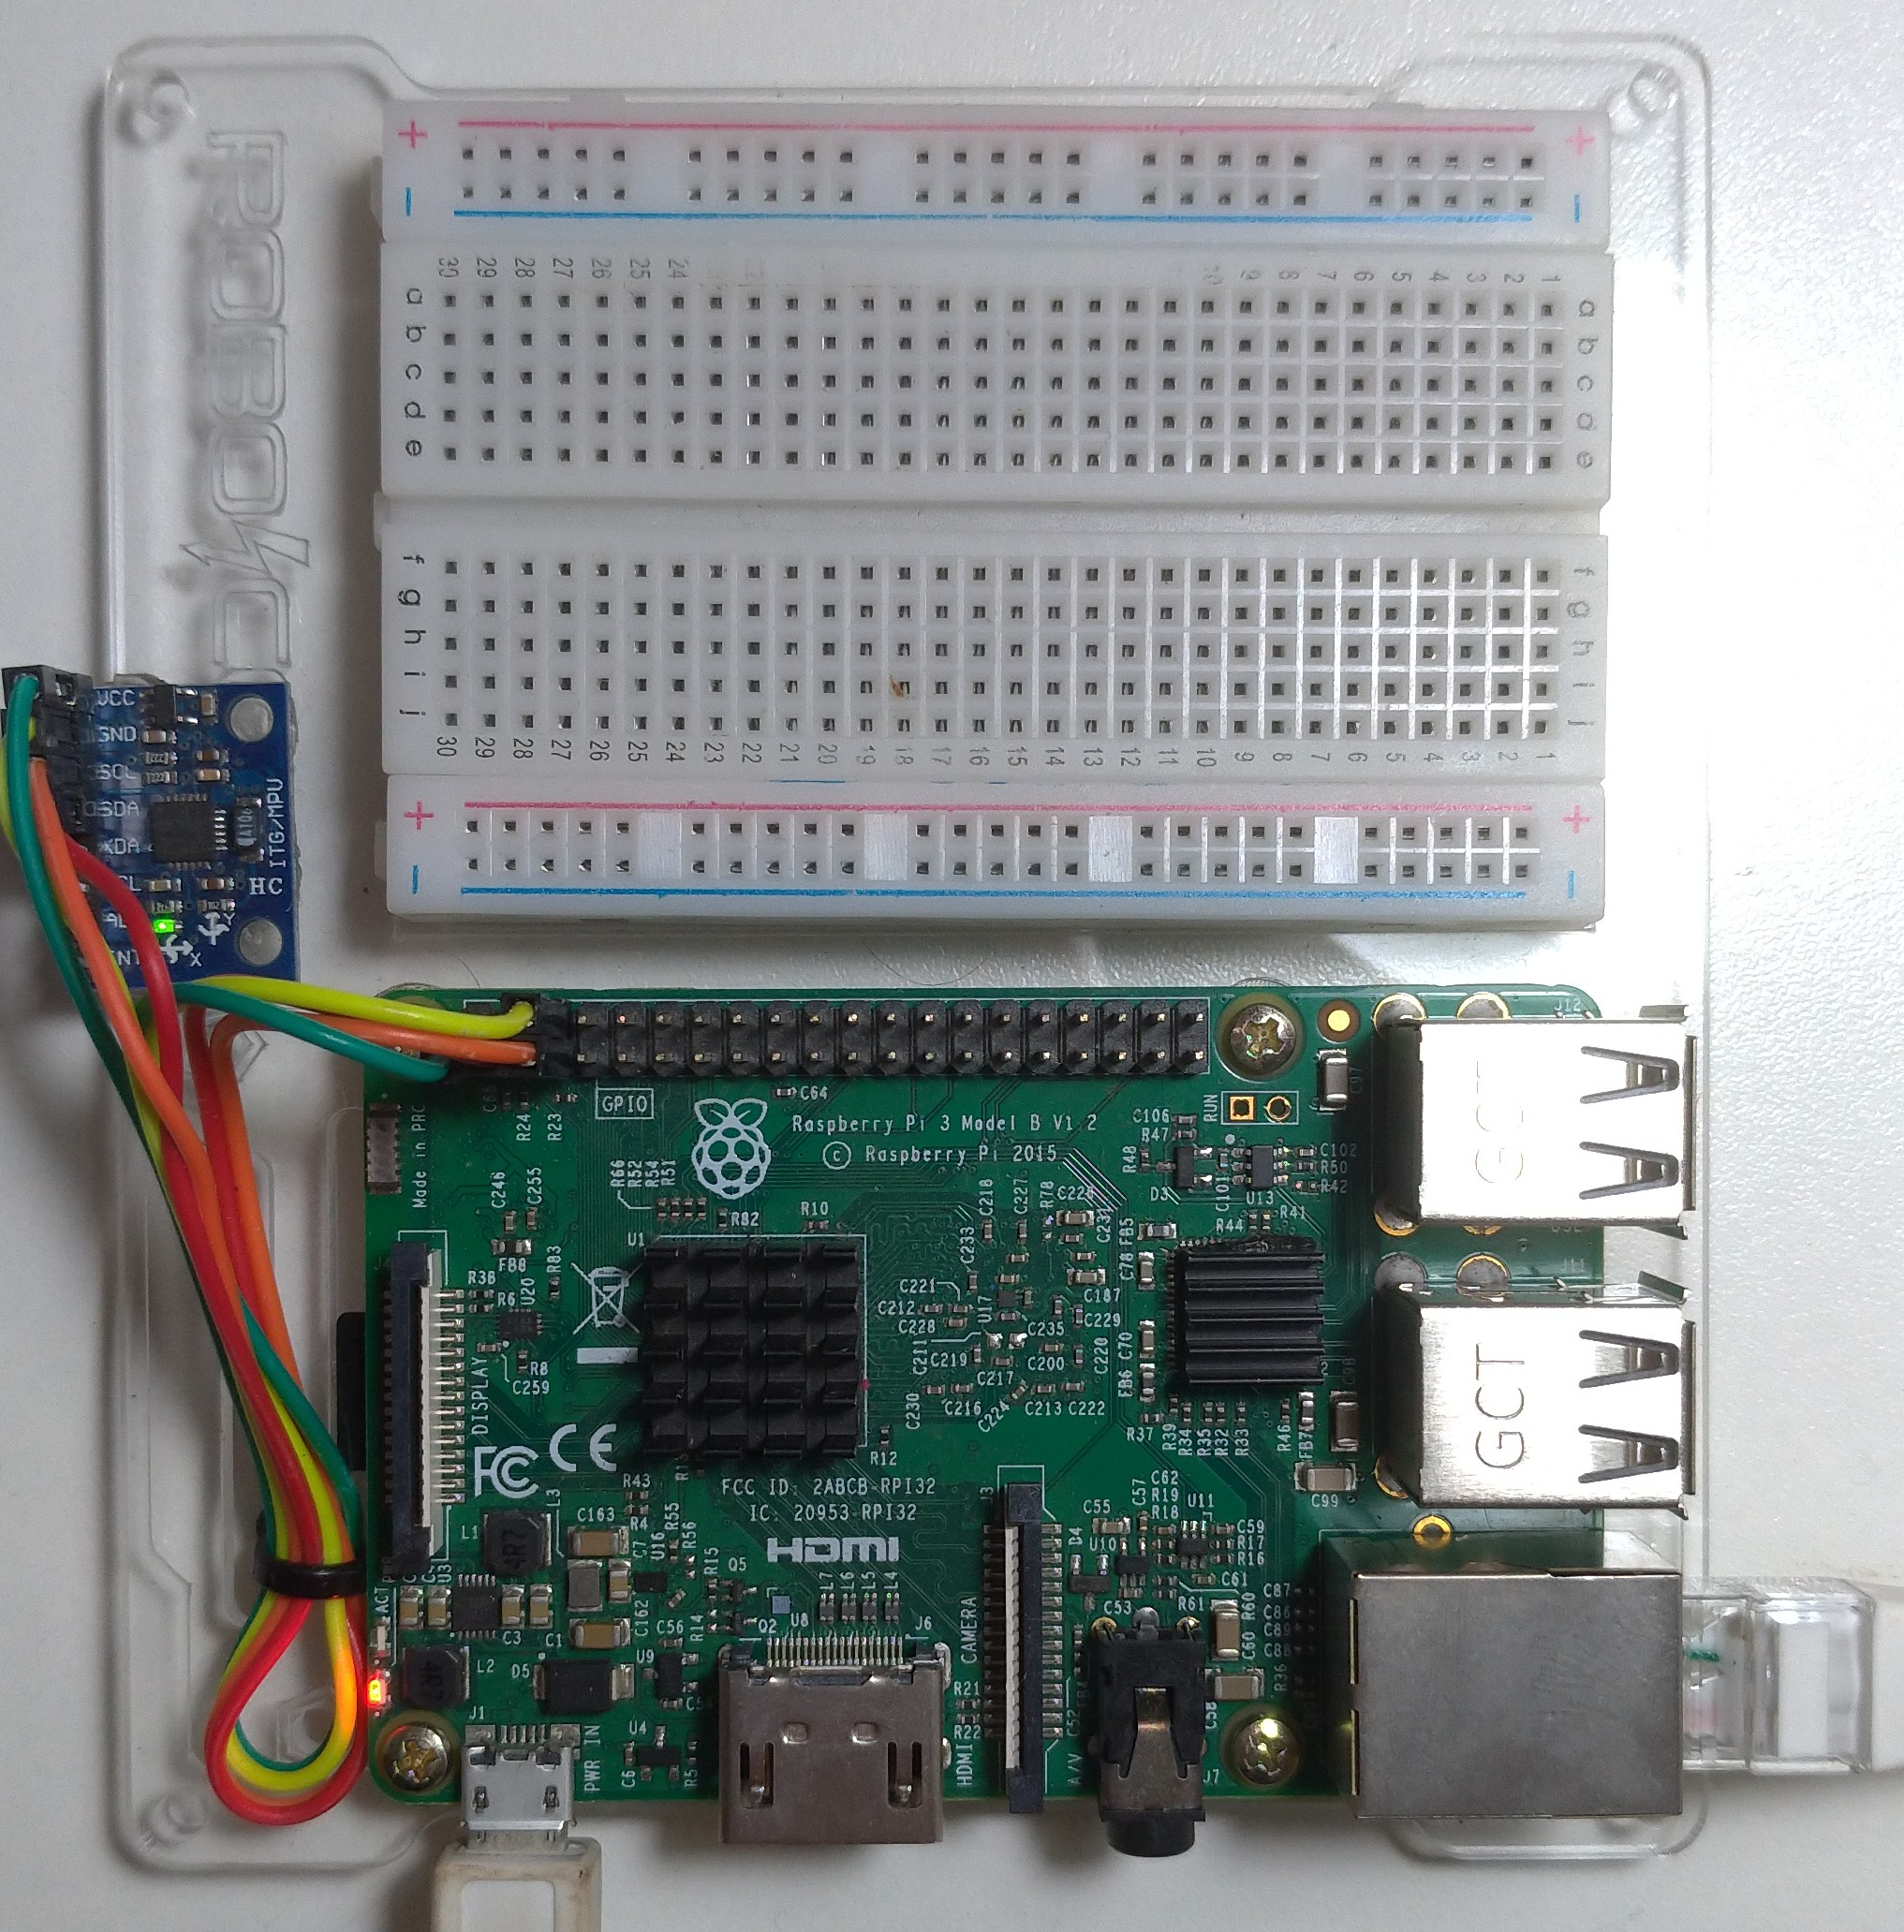
\includegraphics[width=0.5\textwidth]{figuras/mpu6050-proto-top.jpg}
    \fonte{o autor}
\end{figure}

Para a programação Utilizamos programação linguagem C para sistema Linux, com metologia ágil e desenvolvimento em código aberto.

\section{Desenvolvimento de Software}

Após revisão da literatura científica e técnica, estabelecemos os requisitos do software para obtenção de dados úteis dos sensores e os cuidados necessários. Com os requisitos, partimos para codificação em ciclos iterativos com testes, até a satisfação dos requisitos. O produto do desenvolvimento ficará disponível para colaboração e análise.

\section{Testes de bancada para coleta de dados}

Após ciclos de desenvolvimento do código, formulamos testes simples sob condições controladas para obter os dados dos sensores. Os testes consistem em provocar o movimento do corpo do sensor mediante um movimento controlado, por uma distância predeterminada. Nossos sistema de referencia consiste em uma bancada com um braço robótico capaz de fazer os movimentos controlados com precisão. Os testes consistem em um testes estáticos onde o sensor fica parado numa pose determinada por um período fixo de tempo, e testes cinemáticos onde o corpo dos sensores será movimentado em um percurso muito simples cujos dados esperados podemos calcular.

\section{Análise dos dados}

Por último, iremos apresentar os resultados e analisaremos os dados obtido, especialmente na relação entre os resultados esperados e os resultados obtidos. No encerramento ponderamos as causas e eventuais tratamentos posteriores dos resultados.
